\subsection{WYSIWYG}\label{wysiwyg}
�WYSIWYG� staat voor �What You See Is What You Get�. Deze functionaliteit maakt tekst opmaken en verwerken erg gemakkelijk.

\subsubsection{Koptitels}
\begin{enumerate}
\item Ga met de tekstcursor in de regel staan die een Kop 2 of Kop 3 (subkop) moet worden.
\item Klik op het Opmaak openklapmenu en kies Kop 2 of Kop 3.
\end{enumerate}
Het is niet toegestaan om een heading 1 te gebruiken. Volgens de webrichtlijnen is een Kop 1 altijd de paginatitel en komt deze maar 1 keer voor op een pagina. Het gebruik van koppen in teksten dient echter wel op een juiste manier te gebeuren. Gebruik niet de Vet (Bold) knop maar de Opmaak knop. Voor de hoofdkoppen in de tekst gebruikt u Kop 2. Indien hieronder nog subkoppen gemaakt moeten worden gebruikt u Kop 3.

\begin{center}
	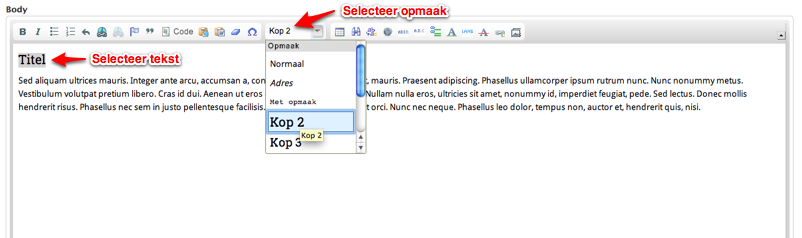
\includegraphics[scale=.7]{img/koptitels.png}
\end{center}

\subsubsection{Bold}
Om een bepaald woord nadruk te geven kan men de Vet (B) knop gebruiken. Gebruik deze knop niet om Headers cq koptitels te maken.
\begin{enumerate}
\item Selecteer het woord met de muis wat u vet wilt maken.
\item Klik op de B-knop.
\item Wilt u het woord niet meer vet hebben, klik dan nog een keer op de B-knop
\end{enumerate}

\begin{center}
	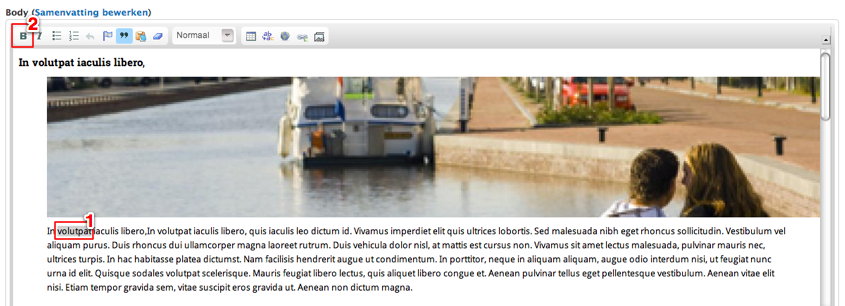
\includegraphics[width=\textwidth]{img/bold.png}
\end{center}

\subsubsection{Italic}
Om een bepaald woord nadruk te geven kan men de Schuin knop gebruiken, oftewel de I-knop.
\begin{enumerate}
\item Selecteer het woord met de muis wat u schuin wilt maken.
\item Klik op de I-knop.	
\item Wilt u het woord niet meer schuingedrukt hebben, klik dan nogmaals op de I-knop.
\end{enumerate}

\begin{center}
	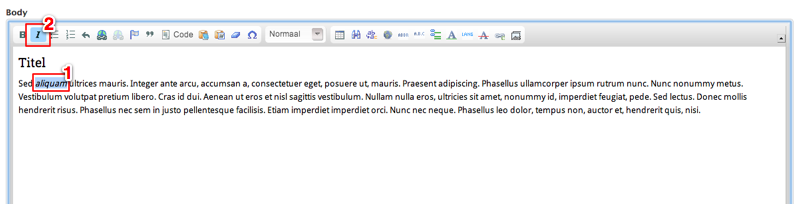
\includegraphics[width=\textwidth]{img/schuin.png}
\end{center}

\subsubsection{Opsomming}
Om een opsomming te maken kan men de Opsomming knop gebruiken.
\begin{enumerate}
\item Klik op de opsomming knop, en voer uw tekst direct in.
\item Om een nieuwe opsommingspunt te gebruiken drukt u op de Enter toets, druk 2 maal op de Enter toets om uit de opsomming te gaan.
\end{enumerate}

\begin{center}
	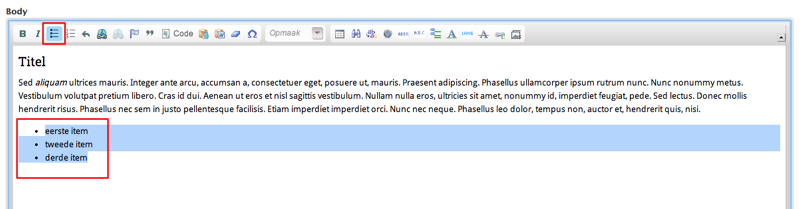
\includegraphics[width=\textwidth]{img/opsomming.png}
\end{center}

\subsubsection{Genummerde lijst}
Om een genummerde lijst te maken kan men de Genummerde lijst knop gebruiken.
\begin{enumerate}
\item Klik op de genummerde lijst knop, en voer uw tekst direct in.
\item Om een nieuw getal te gebruiken drukt u op de Enter toets, druk 2 maal op de Enter toets om uit de genummerde lijst te gaan te gaan.
\end{enumerate}

\begin{center}
	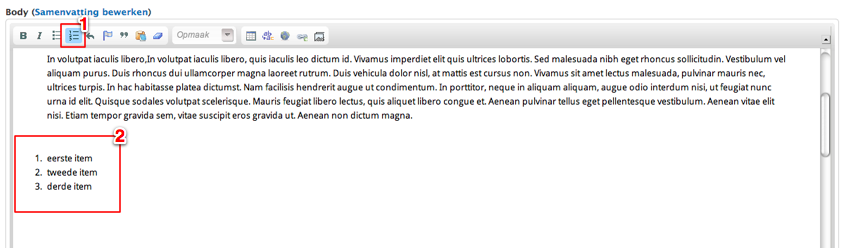
\includegraphics[width=\textwidth]{img/genummerde_lijst.png}
\end{center}

\subsubsection{Iframes}
Om een andere website te tonen op \drupalpath maken we gebruik van een iframe. Via de \emph{wereldbolknop} in 
de WYSIWYG-editor kun je een (externe)pagina tonen op een pagina van \drupalpath. Er zijn drie velden verplicht:
\begin{enumerate}
\item URL
\item Breedte
\item Hoogte
\end{enumerate}

\begin{center}
	
\includegraphics[width=\textwidth]{img/iframe1.png}
\end{center}

\subsubsection{Tabellen}
Via de tabel knop kan een tabel worden ingevoegd. Via de dropdown koppen kan gekozen worden of de rij of kolom of beide.
\begin{center}
	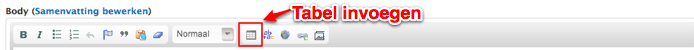
\includegraphics[scale=0.5]{img/tabellen1.png}
\end{center}

\subsubsection{(Externe)Links}
De Linkit module zorgt voor een makkelijke methode om links in content te plaatsen.  

Er zijn twee methoden beschikbaar om links in content te plaatsen. \emph{Methode 1} maakt het mogelijk hele woorden of zinnen naar een (externe)pagina te linken. \emph{Methode 2} maakt het mogelijk een \emph{harde link} te plaatsen; de link is met deze methode is dan gelijk aan het opgegeven pad(URL), de bijbehorende afbeelding zal dit visueel uitleggen. Indien je met \emph{methode 2} een link maakt naar een \emph{interne pagina} dan zal de titel van pagina gebruikt worden voor de klikbare link. 

\textbf{Methode 1:} 

\begin{enumerate}
\item Selecteer het woord of de zin die je wilt \emph{linken}
\item Druk op het \emph{Linkit} knopje
\item Zoek in het eerste veld op interne content, indien gevonden, klik op de gevonden titel
\item Indien je zelf een URL wil invullen, bijvoorbeeld een externe, vul deze dan in bij het veld \emph{Link-url} 
\item Klik op de knop \emph{Link invoegen} om te link toe te voegen aan de content
\end{enumerate}

\begin{center}
	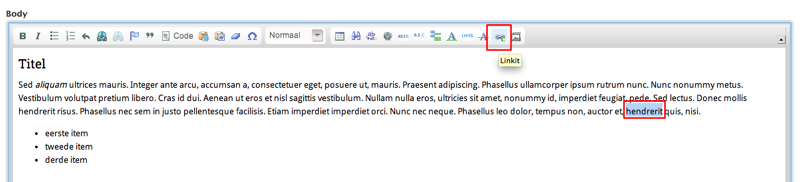
\includegraphics[width=\textwidth]{img/linkit1.png}
	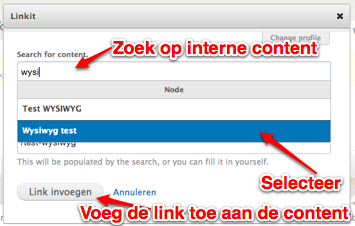
\includegraphics[width=\textwidth]{img/linkit2.png}
	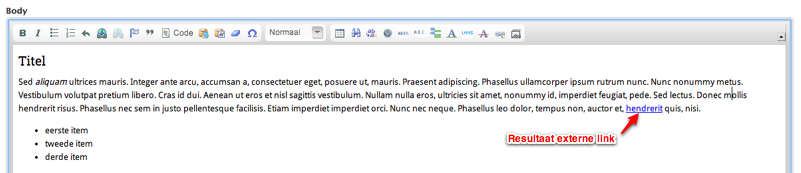
\includegraphics[width=\textwidth]{img/linkit3.png}
\end{center}

\textbf{Methode 2:} 

\begin{enumerate}
\item Druk op het \emph{Linkit} knopje
\item Zoek in het eerste veld op interne content, indien gevonden, klik op de gevonden titel
\item Indien je zelf een URL wil invullen, bijvoorbeeld een externe, vul deze dan in bij het veld \emph{Link-url} 
\item Klik op de knop \emph{Link invoegen} om te link toe te voegen aan de content
\end{enumerate}

\begin{center}
	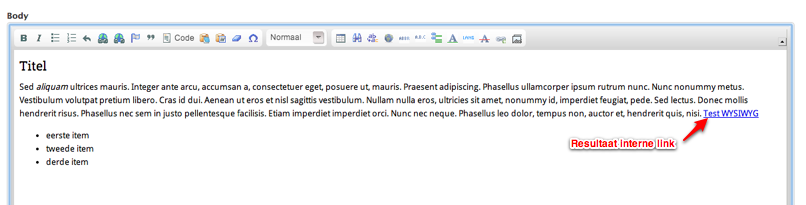
\includegraphics[width=\textwidth]{img/linkit4.png}
	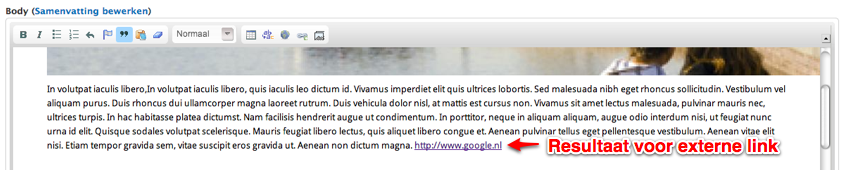
\includegraphics[width=\textwidth]{img/linkit5.png}
\end{center}

\subsubsection{YouTube Embed via WYSIWYG}
\begin{enumerate}
\item Klik op de media button
\item Vul de volledige YouTube url in
\item Klik op de knop \emph{Indienen}
\item Kies vervolgens bij \emph{display as} voor origineel
\item Klik op de knop \emph{Indienen} om de Youtube video in de tekst te plaatsen.
\end{enumerate}

\begin{center}
	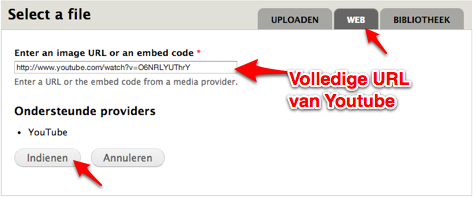
\includegraphics[width=\textwidth]{img/youtube0.png}
\end{center}

\subsubsection{YouTube Embed via Full HTML}
Let op: alleen eindredacteuren kunnen Full HTML nodes wijzigen.
\begin{enumerate}
\item Kopieer de iframe-insluitcode van Youtube.
\item Ga naar de node waarin je een Youtube video wil embedden.
\item Selecteer bij tekstopmaak \emph{Plain text}.
\item Plak de gekopieerde iframe-insluitcode op de plek waar je de Youtube video wil embedden.
\item Selecteer bij tekstopmaak \emph{Full HTML}.
\item Voer eventueel andere wijzigingen door en klik vervolgens onderaan de pagina op de knop \emph{Opslaan}.
\end{enumerate}

\begin{center}
	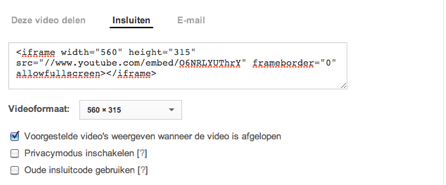
\includegraphics[width=\textwidth]{img/youtube1.png}
	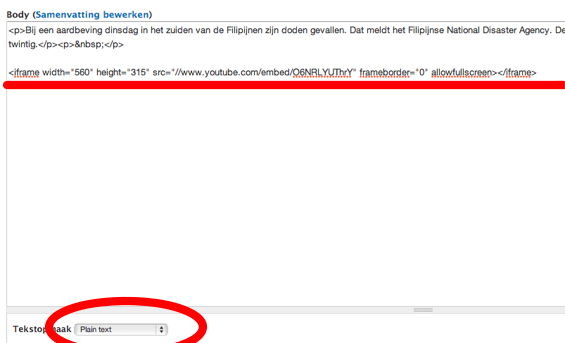
\includegraphics[width=\textwidth]{img/youtube2.png}
	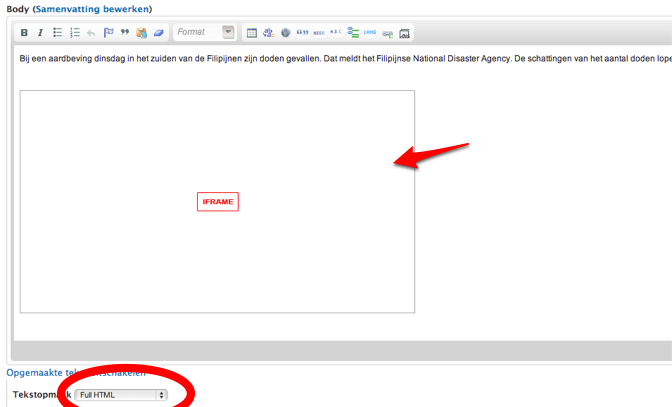
\includegraphics[width=\textwidth]{img/youtube3.png}
\end{center}

\subsubsection{Media}

\begin{center}
	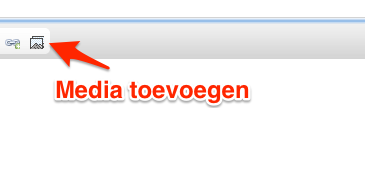
\includegraphics[width=\textwidth]{img/wysiwyg_add_media.png}
\end{center}

Voor het toevoegen van media via de WYSIWYG editor kan je dezelfde stappen volgen als voor \emph{Media}\seeone{media}. Het enige verschil is dat na het selecteren van de afbeelding er gekozen kan worden voor een afbeeldingsformaat, deze staan beschreven in hoofdstuk \emph{Afbeeldingsstijlen}\seeone{afbeeldingsstijlen}. De afbeelding met het gekozen formaat zal altijd links uitlijnen met een marge aan de rechterkant.